%-------------------------------------------------------------------------------
% Kyle Westfall
% westfall@ucolick.org
% UCO/Lick Observatory
% University of California, Santa Cruz
% 1156 High St.
% Santa Cruz, CA 95064
% USA
%
% VERSION:
%       05 Feb 2017: (KBW) v01: stab in the dark
%       01 Aug 2017: (KBW) edits and summary of todo tasks
%
% SUBMITTED:
%
%-------------------------------------------------------------------------------

%\input{../dm_nomenclature/dmnom_rv4.tex}

\documentclass[apj,iop,revtex4,numberedappendix]{emulateapj}
\RequirePackage{calc}
\usepackage{natbib}
\usepackage{url}
\usepackage{amsmath}
\usepackage{mathrsfs}
\usepackage{graphicx}
\usepackage{color}
\bibliographystyle{apj}

\slugcomment{Draft: 22 Jan 2018}

% Some fancy commenting
\definecolor{todo}{RGB}{200,0,0}
\newcommand{\comment}[2][todo]{{\color{#1}[[{\bf #2}]]}}

% Some shorthands
\newcommand{\kms}{{km$~\!$s$^{-1}$}}
\newcommand{\nsaz}{$z_{\rm NSA}$}
\newcommand{\halpha}{H$\alpha$}

\shortauthors{Westfall et al.}
\shorttitle{Asymmetric Drift across the Blue Cloud}

\begin{document}

\title{ Trends in asymmetric drift across the blue cloud }

\author{ Kyle B. Westfall\altaffilmark{1}, Matthew A.
Bershady\altaffilmark{2}, Kevin Bundy\altaffilmark{1}, et al. }

\altaffiltext{1}{University of California Observatories, University of
California Santa Cruz, 1156 High St., Santa Cruz, CA 95064, USA}

\altaffiltext{2}{Department of Astronomy, University of Wisconsin--Madison, 475
N. Charter St., Madison, WI 53706, USA}

\email{westfall@ucolick.org}

% Project collaborators: Matthew Bershady, Anne-Marie Weijmans, Karen
% Masters, Michael Merrifield, Jo Bovy, Kevin Bundy, Niv Drory, Thomas
% Martinsson, Joel Brownstein, Daniel Thomas, Dmitry Bizyaev, David Law,
% Andres Meza, Aaron A. Dutton

\begin{abstract}

Asymmetric drift (AD) is the lag of the mean rotation velocity of the
stellar disk behind the circular speed defined by the total
gravitational potential.  Although it is often considered a nuisance
correction one must apply in circular-speed calculations, the direct
connection between AD and the stellar phase-space distribution function
makes it an interesting dynamical property of galaxies in and of itself.
The SDSS-IV/MaNGA survey provides more than an order of magnitude
increase in any galaxy sample size useful for AD measurements.  In this
pilot study, we measure AD --- or more precisely the differential
tangential lag between the stellar component and \halpha-emitting gas
--- in a set of galaxies with \halpha\ and stellar velocity fields that
are well-fit by simple disk models.  We describe our fitting approach
and the selection of our subsample in detail.  Our final sample of
$\sim$XXX galaxies shows a clear correlation between absolute $i$-band
magnitude and AD measured at effectively all radii.  \comment{The rest
neesds to be updated.} Removing the primary dependence on the rotation
speed, we find that the stellar disk rotation is 90\% of the \halpha\
rotation speed, in the mean.  Our sample size allows us to infer a weak,
yet statistically significant, trend with galaxy $N-r$ color such that,
in the mean, redder galaxies have moderately larger AD relative to their
rotation speeds.  Within the context of an albeit strong set of
assumptions, including a direct proportionality between AD and stellar
velocity dispersion as seen in the Milky Way, we argue that our results
suggest little variation in the mean disk mass-to-light ratio as a
function of absolute magnitude and only modest variations with galaxy
color \comment{last sentence TBD; is Figure 3 consistent with SPS
variations?}.

\end{abstract}

\keywords{ galaxies: kinematics and dynamics --- galaxies: spiral ---
galaxies: structure }

\section{ Motivation }
\label{sec:intro}

For ensembles of stars in a galaxy disk, \citet[][Section
4.4.3]{2008gady.book.....B} provide an intuitive description of
asymmetric drift (AD).  The combined effect of the radially decreasing
surface-density and velocity-dispersion profiles, typical of
axisymmetric systems like the Milky Way, leads to an asymmetric velocity
distribution function with a mean value less than the circular speed
defined by the gravitational potential.  The standard mathematical
representation of this is derived by taking the $v_R$ moment of the
collisionless Boltzmann equation to find the Jeans equation
\citep{Jeans1919} that directly relates the circular speed ($v_c$), the
mean stellar tangential speed ($\overline{v_\theta}$), and the stellar
velocity ellipsoid (SVE) as a function of radius in the plane of
symmetry:
%
\begin{equation}
%
v_c^2 - \overline{v_\theta}^2 = \sigma_R^2\left[
\frac{\sigma_\theta^2}{\sigma_R^2} -
\frac{R}{\rho\sigma_R^2}\frac{\partial(\rho\sigma_R^2)}{\partial R} -
1\right] - R\frac{\partial\overline{v_R v_z}}{\partial z},
%
\label{eq:adformal}
%
\end{equation}
%
where $R,\theta,z$ are the cylindrical coordinates, $\rho$ is the volume
density, and $\sigma$ is the velocity dispersion.  Along with the
standard assumptions of dynamical equilibrium and negligible radial and
vertical flows inherent to its derivation, equation \ref{eq:adformal} is
often simplified by assuming the right-most term is negligible
\citep[cf.][]{1991ApJ...368...79A}; i.e., there is negligible covariance
between the radial and vertical motions as a function of perpendicular
distance to the plane of symmetry.

Asymmetric drift has been measured in numerous systems, perhaps most
notably in the Galaxy.  For example, \citet{1998MNRAS.298..387D} have
shown that populations of stars show a direct correlation between their
velocity dispersion and the degree to which their mean rotation speed
lags behind that of the Local Standard of Rest (LSR), much in line with
the expectation provided by equation \ref{eq:adformal} (see also
\comment{more recent RAVE and RAVE+Gaia references}).

Asymmetric drift measurements in extragalactic systems are common in the
literature \comment{examples}; however, it is most often cast as a nuisance
phenomenon that one must correct for when constructing circular-speed
curves \comment{refs}.  The ubiquity and phenomenology of AD as a
salient observable has not yet been studied for a statistically
significant population of galaxies.  Our aim is therefore to provide a
first look at the correlation between AD measurements and basic
broad-band photometric properties for a large sample of galaxies.

%%%%%%%%%%%%%%%%%%%%%%%%%%%%%%%%%%%%%%%%%%%%%%%%%%%%%%%%%%%%%%%%%%%%%%%%
\begin{figure*}
%
\begin{center}
%
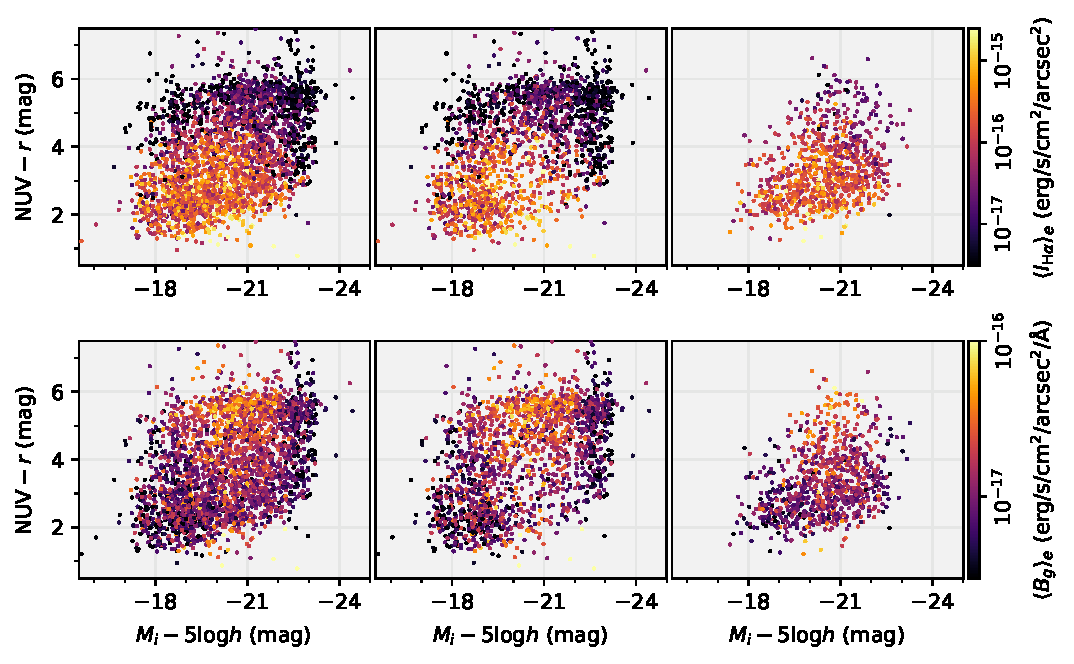
\includegraphics[width=0.9\textwidth]{figs/cmd_flux.pdf}
%
\end{center}
%
\caption{
%
${\rm NUV} - r$ color and absolute $i$-band magnitude ($M_i$) from the
NASA-Sloan Atlas (NSA) for all galaxies observed during the first two
years of the MaNGA Survey (left), the subsample of galaxies {\em not}
selected to be kinematically regular (middle; see text), and the AD
sample used throughout the remainder of our analysis.  The color of the
data points in the top row represent the mean \halpha\ surface
brightness within the elliptical-Petrosian half-light radius according
to the colorbar to the right; the bottom row replaces the color by the
mean $g$-band surface brightness density over the same elliptical
aperture.
%
}
%
\label{fig:sample}
%
\end{figure*}
%%%%%%%%%%%%%%%%%%%%%%%%%%%%%%%%%%%%%%%%%%%%%%%%%%%%%%%%%%%%%%%%%%%%%%%%

In addition to a basic characterization of the phenomenon, our interest
in AD stems from its fundamental dynamical connection to the full
phase-space distribution function of a galaxy's stars, as empirically
demonstrated in the Milky Way.  Indeed, \citet{2011ApJ...742...18W} used
AD to constrain the axial ratios of the SVE given direct measurements of
the line-of-sight (LOS) stellar velocity dispersion, $\sigma$.
Alternatively, if one can statistically constrain the shape of the SVE
\citep[e.g.][]{2012MNRAS.423.2726G}, measurements of AD could then be
used as a proxy for stellar $\sigma$ via equation \ref{eq:adformal}.
Such an AD-$\sigma$ relation becomes attractive in the
low-surface-brightness and low-velocity-dispersion regimes where direct
measurements of $\sigma$ are difficult and/or expensive.  Adopting this
paradigm outright, we define $\sigma_a^2 \equiv v_c^2 -
\overline{v_\theta}^2$, following from equation \ref{eq:adformal}, for
use throughout this paper.

For disk galaxies, there is a decades-long industry of using cold-gas
tracers to construct circular-speed curves of galaxies \comment{refs}.
These data have provided the first concrete arguments for the presence
of massive dark-matter halos \comment{ref} based on mass-model
reconstruction \comment{refs} and have formed the basis for the most
robust Tully-Fisher relations compiled for the local Universe
\comment{refs}.  However, it is important to acknowledge that one cannot
directly measure $v_c$, effectively making $\sigma_a$ unobservable.
That is, every tracer has some non-zero dynamical pressure such that it
will lag behind the theoretically defined circular speed.  There are
very clear examples of early-type galaxies that show differential AD in
their molecular (e.g., CO), atomic (e.g., \ion{H}{1}), and/or ionized
(\halpha) tracers relative to a robust mass model of $v_c$
\citep{2013MNRAS.429..534D} due to the different turbulent/thermal
pressures intrinsic to these tracers.  However, these signatures are
much less apparent in disk galaxies.  For example,
\citet{2013A&A...557A.131M} show that \halpha\ and \ion{H}{1} rotation
curves are consistent for the DiskMass Survey within the limits of their
constraints on beam-smearing.  This suggests that any correction for the
lag behind the circular speed of either the \halpha- or
\ion{H}{1}-emitting gas should be small.  Indeed, theoretical
calculations \citet{2010ApJ...721..547D} suggest that gas-pressure
corrections to \ion{H}{1} rotation curves should be largely negligible
for galaxies with circular speeds larger than roughly 75 \kms.
Nevertheless, we emphasize here that our measurements of $\sigma_a$ may
be better termed as a {\em differential tangential lag} because they are
calculated as the quadrature difference between the {\em observed}
\halpha\ and stellar rotation curves in our galaxy sample (Section
\ref{sec:data}).  These measurements are perfectly valid in their own
right; however, their interpretation in the context of the theoretical
definition of AD must be done with care, as we discuss in Section
\ref{sec:discussion}.

\comment{Outline should be updated} We present the data used for our
analysis in the following section.  Section \ref{sec:results} presents
the strong correlation seen in out galaxy sample between the absolute
$i$-band magnitude and AD signal measured at half of an effective radius
(0.5 $R_{\rm eff}$).  We also illustrate the weak color dependence in
this relation.  Finally, we summarize and discuss these results in
Section \ref{sec:discussion}.  \comment{flesh out}

\section{Data}
\label{sec:data}

\subsection{Galaxy Sample}

We use integral-field spectroscopy from the SDSS-IV/MaNGA (Mapping
Nearby Galaxies from APO) Survey to construct stellar and ionized-gas
velocity fields for 2715 unique galaxies, 39 of which have multiple
observations.  These data were obtained during the first two years of
normal survey operations, and the reduced datacubes are included in DR14
\citep{2017arXiv170709322A}.  \comment{additional references to
technical papers}.

The MaNGA galaxy selection is discussed in detail by
\citet{2017AJ....154...86W}; the galaxies in DR14 represent a random
sampling of full MaNGA parent sample.  The parent sample is selected
using simple cuts in absolute $i$-band magnitude, $M_i$, and redshift,
$z$, from the NASA-Sloan Atlas (NSA; \url{www.nsatlas.org}) to produce
two main galaxy samples, Primary and Secondary, with roughly twice as
many galaxies observed from the former.  The main distinguishing
characteristic of the two samples is MaNGA provides uniform coverage to
$\sim$$1.5R_e$ and $\sim$$2.5R_e$ for the Primary and Secondary sample,
respectively.  The Primary sample is supplemented by a
``Color-enhanced'' sample that improves coverage of the galaxy
population in low-density regions of color-magnitude space; the
combination of Primary and Color-enhanced samples are referred to as the
Primary$+$ sample.  Although we will comment on any difference in our
analysis results between the Primary$+$ and Secondary samples, we
largely treat these two samples identically in our analysis.

The ($N-r, M_i$) color-magnitude diagram (CMD) for MaNGA galaxies in
DR14 (using NSA photometry) is shown in the left-most panels of Figure
\ref{fig:sample}.  Data in the top and bottom row are colored according
to, respectively, the average \halpha\ surface brightness and
$g$-band-weighted mean flux density within 1 $R_e$.  We discuss Figure
\ref{fig:sample} in the context of our selection of galaxies appropriate
for our AD analysis \comment{below}.

\subsection{MaNGA Spectroscopy}

The MaNGA fiber-feed system \citet{2015AJ....149...77D} for the
2.5-meter Sloan telescope at Apache Point Observatory (APO) is coupled
to the SDSS-III/BOSS spectrographs \citep{2013AJ....146...32S}, a pair
of dual-channel spectrographs that provide $R_\lambda =
\lambda/\Delta\lambda \approx 2000$ across the full spectral range of
$3600\AA \lesssim \lambda \lesssim 10300\AA$.  Each MaNGA pointing
provides simultaneous observations of 17 galaxies using fiber bundles
ranging from 19 to 127 fibers.  The dither pattern of the MaNGA
observational strategy \citep{2015AJ....150...19L} provides a remarkably
uniform depth for each observation with fields-of-view ranging from
$12\arcsec$ to $32\arcsec$ for the smallest and largest bundles,
respectively.  The uniform depth yields a tight correlation between flux
density per spaxel and signal-to-noise (S/N); see
\citet{2015AJ....150...19L, 2016AJ....152...83L} and
\citet{2016AJ....151....8Y, 2016AJ....152..197Y} for additional details
about the survey execution and performance.

In particular, \citet{2016AJ....152...83L} describes the methods used by
the MaNGA Data Reduction Pipeline (DRP) is an to produce wavelength-,
flux- \citep{2016AJ....151....8Y}, and astrometrically calibrated
spectra from the raw CCD data.  The reduction procedures are similar to
those used by the SDSS-III/BOSS pipeline, but with significant
adjustments as required by the MaNGA observations.  

Here, we use the rectified datacubes that have been logarithmically
binned in wavelength (i.e., the \verb|LOGCUBE| files).  The MaNGA data
cubes are constructed by regridding the flux of all spectra for a given
plate--IFU combination in each wavelength channel to an on-sky pixel
(spaxel) sampling of $0\farcs5\times0\farcs5$.  The interpolating PSF
used in this process is a two-dimensional Gaussian with a standard
deviation of $0\farcs6$ and a truncation radius of $1\farcs7$.  This
interpolation process leads to significant covariance between the
spaxels in a given wavelength channel \citep{2016AJ....152...83L}.  This
spatial covariance does not affect the primary result of our paper, so
we defer a more detailed consideration of the covariance for future
work.

\subsection{Stellar and Ionized-Gas Kinematics}

The kinematic measurements are determined by a preliminary version
(2.0.2) of the MaNGA Data Analysis Pipeline (DAP; Westfall et al., {\it
in prep}).  The pipeline provides simple single-Gaussian fits to the
\halpha\ emission feature that we use for the ionized-gas kinematics,
and the stellar kinematics are determined using {\tt pPXF}
\citep{2004PASP..116..138C, 2017MNRAS.466..798C}.  The templates used by
{\tt pPXF} are a hierarchically clustered distillation of the MILES
stellar template library \citep{2011A&A...532A..95F}.  We find the
velocity measurements to be statistically well behaved to a $g$-band
signal-to-noise ratio of S/N$\sim$1.\footnote{
%
This and other assessments of the fidelity of the stellar kinematics
provided by the DAP will be discussed in detail by Westfall et al., {\it
in prep}.}
%
Therefore, we perform our analysis using the spaxel-by-spaxel
determination of the stellar and ionized-gas kinematics.\footnote{
%
However, note that only the stellar kinematic determined for data
Voronoi binned to S/N$\sim$10 will be provided as part of DR15.}


\section{Velocity-Field Modeling}

\subsection{Formalism}

We fit the \halpha and stellar velocity fields using an approach similar
to \citet{2013ApJ...768...41A} \citep[][see also
\citealt{2011ApJ...742...18W}].  The velocity field is modeled as an
infinitely thin disk in fully circular rotation that follows a
parameterized form $V_{\rm rot}(R)$; here we use a simple hyperbolic
tangent function:
%
\begin{equation}
%
V_{\rm rot}(R) = V_\infty \tanh(R/h_{\rm rot}),
%
\label{eq:tanh}
%
\end{equation}
%
where $V_\infty$ is the asymptotically flat rotation speed and $h_{\rm
rot}$ is a characteristic scale for the rise of the rotation curve, and
the model line-of-sight (LOS) velocity is
%
\begin{equation}
%
V_{\rm los}(x,y) = V_{\rm rot}(R[x,y])\ \cos(\theta[x,y])\ \sin i +
V_{\rm sys}
%
\label{eq:vlos}
%
\end{equation}
%
where $i$ is the disk inclination (a ``face-on'' disk has $i=0$), and
$V_{\rm sys}$ is the systemic velocity of the galaxy.  The disk-plane
polar coordinates ($R,\theta$) in Equation \ref{eq:vlos} are functions
of the on-sky position:
%
\begin{eqnarray}
%
x_d & = & (x+x_0)\sin\phi_0 + (y+y_0)\cos\phi_0 \\
%
y_d\cos i  & = & -(x+x_0)\cos\phi_0 + (y+y_0)\sin\phi_0 \\
%
R^2 & = & x_d^2 + y_d^2 \\
%
\tan\theta & = & -y_d / x_d,
%
\label{eq:diskrt}
%
\end{eqnarray}
%
where ($x,y$) is the on-sky position ($+$$x$ is to the east) relative to
the center of the object as defined by the targeting catalog,
($x_0,y_0$) is the location of this pointing center of the IFU relative
to the dynamical center, $\phi_0$ is the position angle defined from
north through east of the receding side of the major axis, and
($x_d,y_d$) are the disk-plane Cartesian coordinates.  Note that
$\theta=0\arcdeg$ along the major axis on the receding side of the
galaxy. 

\comment{REST IS OLD TEXT}

[[We emphasize that this parametrization is used in the determination of
the kinematic geometry from the rotation curve, but not as measurements
of the rotation speed itself (see Section XX).]]

Provided $j=0...N_{\rm spaxels}$ LOS velocity measurements, $V_{{\rm
los},j}$, and their errors, $\epsilon_{v,j}$, we determine the
best-fitting model velocity field using a Levenberg-Marquardt
minimization algorithm with the following figure-of-merit:
%
\begin{equation}
%
\chi^2 = \sum_j \frac{ (V_{{\rm los},j}-V_{\rm mod}[x_j,y_j])^2 }{
\epsilon^2_{v,j} + \epsilon^2_{\rm mod}},
%
\label{eq:vfchi}
%
\end{equation}
%
where $\epsilon_{\rm mod}$ is an intrinsic scatter of the measured LOS
velocities about the simplistic model.  To simplify further discussion,
we denote the $j$ components of the sum on the right-hand of the
equation as $\chi^2_j$. [[Go back and include the ``beam-smearing''
term?]]

In an effort to minimize the well-known covariance between the
inclination and rotation speed (refs), our velocity-field
parameterization actually fits the {\em projected} rotation curve (i.e.,
$V_{\rm rot}(R) \sin i$) instead of the disk-plane rotation speed
itself.  The fitted parameters for a single velocity field are then
$x_c$, $y_c$, $i$, $\phi_0$, $V_{\rm sys}$, $V_\infty \sin i$, and
$h_{\rm rot}$.

\subsubsection{Implementation details}
\label{sec:vfimplement}

The description in Section \ref{sec:vfbasic} [[apart from leaving out
the beam-smearing term]] is identical to the approach of
\citet{2013ApJ...768...41A}.  The alterations specific to our
implementation are as follows \citep[cf.][]{2011ApJ...742...18W}:

\begin{enumerate}
%
\item {\em Simultaneous VF fitting}:  We have extended the code from
\citet{2013ApJ...768...41A} to allow for simultaneous fits to multiple
dynamical tracers, while allowing the rotation curves of the two
components to be different.  Although we do fit the \halpha and stellar
data fit independently, this is primarily used in the selection cuts
imposed in Section \ref{sec:kingeomcuts}.  When fitted simultaneously,
there are three additional free parameters compared to those listed
above: the two additional rotation curve parameters and systemic
velocity of the second dynamical tracer.  That is, even when fitting the
two velocity fields simultaneously, we allow for the systemic velocities
of the two tracers to be different.  This is primarily to allow for,
e.g., systematic errors in the velocity registration of the template
libraries used to determine the stellar kinematics.  Ideally, one would
like to force the systemic velocities of the two tracers to be the same,
and we discuss the effects on our results by allowing them to be
different in Section \ref{sec:kingeom}.
%
\item{\em Intrinsic scatter}:  The intrinsic scatter term,
$\epsilon_{\rm mod}$, serves a number of purposes.  Its effect is to
alter the error-weighted distribution of the fit residuals such that it
closely follows a Gaussian distribution with unity standard deviation;
that is, it forces the reduced $\chi^2$, $\chi^2_\nu$, of the fit to be
very close to unity.  Indeed, \citet{2013ApJ...768...41A} chose
$\epsilon_{\rm mod}$ such that $\chi^2_\nu$$\sim$1 to within 1\%.  Our
approach is to instead iteratively adjust $\epsilon_{\rm mod}$ until the
growth curve of $\chi^2_j$ is marginally different from the growth curve
of a Gaussian function with unity standard deviation.  This approach is
primarily chosen given its advantage in dealing with our third
alteration. [[Affect on formal parameter errors from the covariance
matrix.]]
%
\item{\em Measurement Rejection}:  The fits to the velocity fields
generally provide $\chi^2_\nu > 1$ when $\epsilon_{\rm mod} = 0$,
meaning that there is a general systematic discrepancy of model with
respect to the $V_{\rm los}$ measurements that is not accounted for by
the random errors, $\epsilon_{v,j}$.  Although most of the discrepancies
can be accounted for by a small ($\epsilon_{\rm mod}\sim XX$) scatter
about the simplistic model, systematic error in the kinematic
measurements, particularly at low SNR, can lead to a number of
$V_{{\rm los},j}$ with $\chi^2_j \gg 1$.  We iteratively reject these
data from the fit at the same time as we determine the intrinsic scatter
term, $\epsilon_{\rm mod}$.  After fitting the data with a given
$\epsilon_{\rm mod}$ (starting with 0), we iteratively reject points
with $\chi^2_j > 1$, starting with the largest value, and adjust
$\epsilon_{\rm mod}$ until the root-mean-square difference between the
growth curve of $\chi^2_j$ and a Gaussian with unity standard deviation
is minimized.  This whole process of fitting the velocity field,
determining $\epsilon_{\rm mod}$, and rejecting aberrant data is done
many times to make sure that the points that are rejected and the value
of $\epsilon_{\rm mod}$ is not strongly biased by the initial fit to the
velocity field.
%
\end{enumerate}

% [[I realize that the above two (maybe even all three) things are
% highly detailed.  We probably want to make them simpler.]]

\subsubsection{Initialization}
\label{sec:vfinit}

The MaNGA data cubes (cf. Law et al.~{\em in prep}) provide an accurate
registration of the spectrophotometry with on-sky imaging data to
provide a detailed astrometric calibration in the form of a
world-coordinate system (WCS) in the fits headers. The coordinates of
the targeted galaxy\footnote{
%
This is generally the center of the data cube field-of-view; however,
some observations were purposely offset for testing purposes.
%
} are, in general, exactly the coordinates provided by the NASA-Sloan
Atlas; however, some coordinates have been adjusted to better match the
galaxy center [[check this with David W.]] (cf., Wake et al.~{\em in
prep}).  The ($x,y$) coordinate system in Eqn. \ref{eq:vlos} is then
established by setting the (0,0) coordinate at the galaxy center.  Thus,
when freely fit, we should expect to find $x_0 = y_0 = 0$ arcsec.

The NASA-Sloan Atlas also provides ellipticity and position angle
measurements for isophotal contours of each galaxy, which we use as the
initial guesses for the kinematic inclination and position angle,
respectively.  For an oblate spheroid with intrinsic axial ratio $q_0$
and an observed ellipticity of $\varepsilon = 1-b/a$, its inclination to
the LOS is given by (ref)
%
\begin{equation}
%
\cos^2 i_{\rm phot} = \frac{ (1-\varepsilon)^2 - q_0^2 }{ 1 - q_0^2 }.
%
\label{eq:inc}
%
\end{equation}
%
For our measurements of $i_{\rm phot}$, we assume $q_0 = 1/8$ (Bershady;
but, cf., Weijmanns).

Given that our definition of $\phi_0$ is tied to the vector along the
major axis toward the receding side of the velocity field, the kinematic
position angle has a valid range of $2\pi$.  However, photometric
position angles only have a valid range of $\pi$.  Our initial guess of
$\phi_0$ is either the same as the photometric value or flipped by
$180\degr$ based on an initial deprojection of the rotation speed along
the photometric position angle.

Finally, we use the redshift provided by the NASA-Sloan Atlas as the
initial estimate of the systemic velocity, $V_{\rm sys} = c z_{\rm
NSA}$.

\subsubsection{Fitting iterations}
\label{sec:vfiter}

We expect AD to be present in all galaxies, and so we
attempt to fit all 1392 galaxies in the current MaNGA sample.  For such
a large galaxy sample, it is difficult to attempt human interaction at a
detailed level with each fit.  Therefore, all of the fits have been
performed in an automated way.  To help in the quality assessments of
the fits (Sections \ref{sec:kingeom} and \ref{sec:kingeomcuts}), we fit
the velocity fields of each tracer (\halpha-emitting gas and stars) both
individually and in a single, simultaneous fit.  Additionally, we
perform the individual and simultaneous fits under permutations of
fixing and freeing the inclination and center.

The determination of $V_{\rm sys}$ and $\phi_0$ are generally robust and
well-constrained by the data, meaning there is no need to fix them to
certain values.  Conversely, the inclination and center can be poorly
determined in certain regimes.  For example, when the observed velocity
field is that of a solid-body rotator, the isovelocity contours all
become parallel to the minor axis ($V_{\rm rot} \propto R$ and, at a
fixed perpendicular distance from the minor axis, $\cos\theta \propto
R^{-1}$).  Thus, in the absence of any other information, one could
place the center anywhere in the velocity field without affecting
$\chi^2$.  Similarly, measurements of inclination depend on the
curvature seen in the isovelocity contours and there is no such
curvature for a solid-body rotator.  Finally, at low inclination, the
curvature in the isovelocity contours can be imperceptible due to the
stochastic deviations (random and systematic) about the fitted model.
Therefore, by performing fits that both fix and free the center and
inclination, we can test the consistency of the results and the
significance of kinematically constrained parameters versus simply
adopting the photometric one.

In addition, we impose boundaries on the allowed range for the geometric
parameters.  We force the systemic velocity to be within $\pm1000$
\kms{} of the input guess, we force $0.1\leq i \leq 85$ and
$0\leq\phi_0<360$, and we define a bounding box for the fitted center to
be $\sim$20\% of the full field-of-view.  The limits for the IFUs with
19, 37, 61, 91, and 127 fibers are limited to $\pm1\arcsec$,
$\pm2\arcsec$, $\pm2\arcsec$, $\pm3\arcsec$, and $\pm3\arcsec$,
respectively.

In summary, we perform 12 velocity-field fits for each galaxy: (1) four
fits are permutations of fixing and freeing the center and inclination
and (2) each of these four fits is done when only fitting the \halpha
data, only fitting the stellar data, and fitting both tracers
simultaneously.
%
\begin{figure*}
%
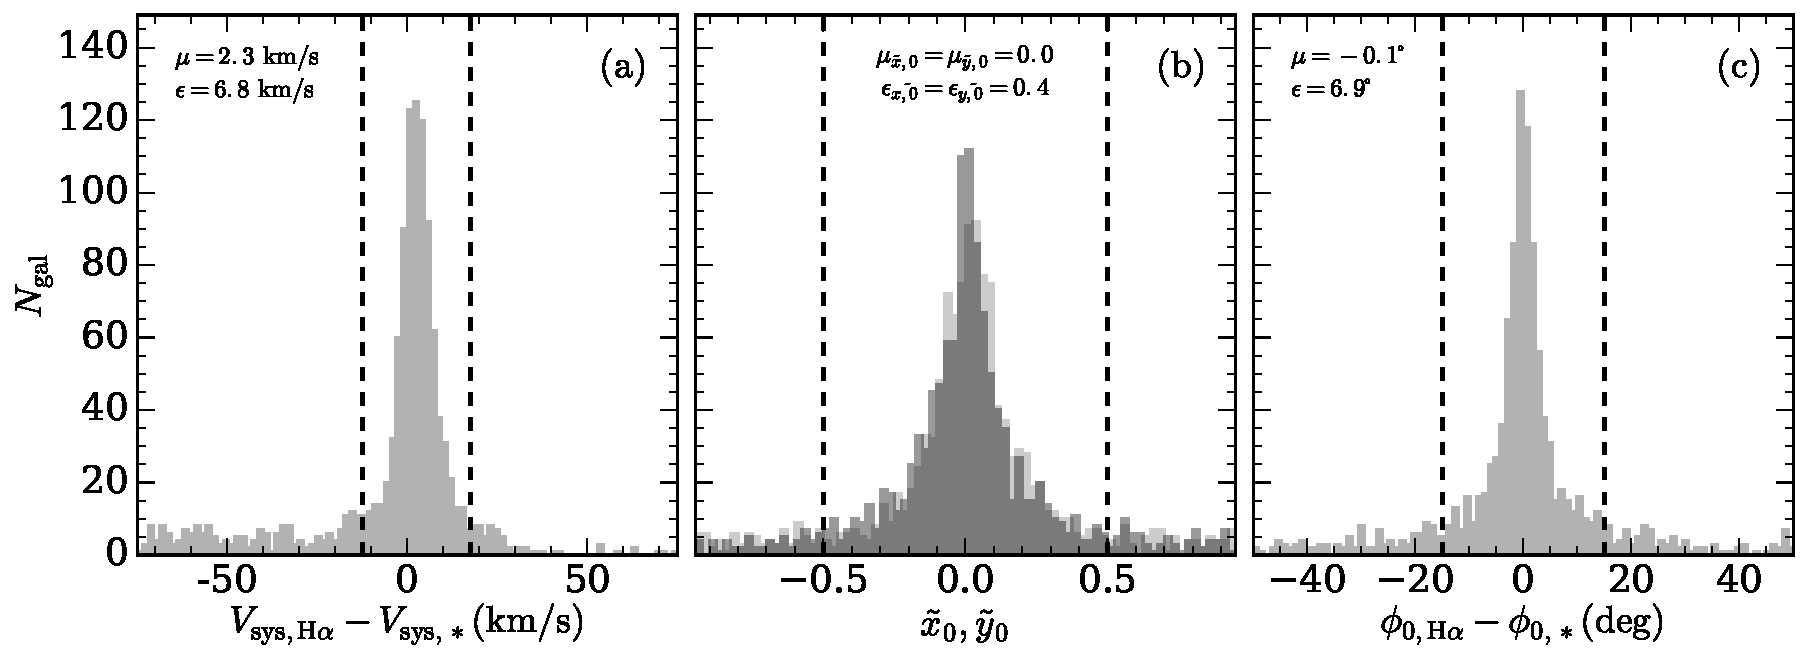
\includegraphics[width=0.9\textwidth]{figs/sys_cen_pa.pdf}
%
\caption{
%
Distribution of (a) the difference between the \halpha and stellar
systemic velocities; (b) the center relative to the imposed fit
boundary; and (c) the difference between the \halpha and stellar kinematic
position angles.  For the center panel, the distributions of
$\tilde{x}_0$ and $\tilde{y}_0$ are shown as (transparent) light and
dark histograms, respectively.  The 3-sigma clipped mean ($\mu$) and
standard deviation ($\epsilon$) for each distribution is provided in
associated panel.  The dashed lines illustrate the cuts that we adopt
for each parameter in our AD analysis(see text).
%
}
%
\label{fig:sys_cen_pa_hist}
%
\end{figure*}

\subsection{Kinematic Geometry Results}
\label{sec:kingeom}

For our AD measurements, we require robustly measured kinematic
geometries that can be applied to both the \halpha-emitting and stellar
components.  This requirement drives our assessments of the kinematic
geometries and the selection of galaxies to propagate through our AD
analysis in the remaining sections of the paper.  For example, it is
physically plausible to find a significant offsets between the position
angles of gas and stars (e.g., Chen et al.; Belfiore et al.); however,
this is typically the signature of an accretion event and not conducive
to an AD measurement.  Given the fits that we have performed, we can
check both the consistency of the \halpha and stellar geometries, as well
as their consistency with the morphological geometry.

We first limit our assessments to those galaxies with successfully
converged velocity-field fits for all 12 fit iterations, which cuts our
sample from 1392 to 1322 galaxies.  [[Should maybe have a sentence about
why these failed?]]  All subsequent cuts include this base-level
selection.

\subsubsection{Systemic velocity}

When fit separately, the best-fitting systemic velocities for both the
\halpha and stellar data are in good agreement with each other and with
the redshifts in the NASA-Sloan Atlas, $cz_{\rm NSA}$.  The mean
difference with respect to $cz_{\rm NSA}$ over the full 1322 galaxies is
less than 10 \kms{} and the standard deviation is approximately the
velocity width of a spectral channel ($\sim$70 \kms{}), regardless of
the fitting constraints or tracer.

The result is approximately the same when considering the difference
between the \halpha-only and stellar-only fit parameters.  Indeed, we
should expect that the systemic velocity should be the same for the
\halpha and stellar components; however, we have allowed them to be
different, even when fitting the two velocity fields simultaneously.
Fig.~\ref{fig:sys_cen_pa_hist}(a) shows the distribution of $V_{{\rm
sys,H}\alpha} - V_{{\rm sys},\ast}$ when both are fit simultaneously.
After applying a 3-sigma clipping algorithm, we find a mean difference
of $2.3\pm6.8$ \kms{}.  It is difficult to understand how this
systematic offset could arise either physically or due to a
wavelength-calibration error.  We therefore assume that this mean offset
is due to a systematic error in the velocity registration of the MIUSCAT
template spectra across our fitted wavelength range.  Further work is
required to exactly address this problem; however, it has a minimal
effect on our analysis [[need to test this]].

To avoid the strong outliers, particular toward the negative end of
Fig.~\ref{fig:sys_cen_pa_hist}(a), we select only those galaxies with
-12.5 \kms{} $\leq V_{{\rm sys,H}\alpha} - V_{{\rm sys},\ast} \leq 17.5$
\kms{} for further analysis; 850 of 1322 galaxies (64\%) meet this
criterion.

\subsubsection{Pointing relative to the dynamical center}

In Section \ref{sec:vfiter}, we noted that the pointing relative to the
dynamical center ($x_0,y_0$) has a bounding box placed on it that is
IFU-dependent.  When selecting results for our AD analysis, we care more
about the fitted center relative to the bounding box than we do about
the absolute center in arcseconds.  Therefore, in
Fig.~\ref{fig:sys_cen_pa_hist}(b) we show the ratio of the fitted center
relative to the size of the bounding box --- e.g., $-1\leq \tilde{x}_0
\leq 1$ --- for both on-sky coordinates.  Recall (Section
\ref{sec:vfbasic}) the definition of our ($x,y$) coordinate system is
such that a result of $(x_0,y_0) = (0,0)$ means that the morphological
and dynamical centers are co-located.

The results in Fig.~\ref{fig:sys_cen_pa_hist}(b) are specifically for
the case where we have fit both tracers simultaneously.  We find that
the simultaneous fit to both tracers reduces the scatter about the
morphological center compared to the result for the fits to an
individual tracer: the standard deviations are 0.52, 0.44, and 0.39 for
the \halpha, stellar, and combined fits, respectively.  Under the
expectation that the morphological and dynamical centers should be the
same for dynamically settled galaxies, we force both $\tilde{x}_0$ and
$\tilde{y}_0$ to be within $\pm0.5$, of which 926/1322 (70\%) of the
galaxies satisfy.  Before applying this selection, the standard
deviation of $(x_0,y_0)$ is approximately $0\farcs9$ for each
coordinate, which is reduced by a factor of 3 for the selected sample of
926 galaxies.

\subsubsection{Position angle}

The kinematic position angle is periodic with an imposed range in the
fit of $0\leq\phi_0\leq360$.  In calculating the difference between any
two position angles, we account for this range and periodicity such that
the difference in position angle should be centered at $0\degr$, as is
the case when comparing $\phi_{0,{\rm H}\alpha}$ and $\phi_{0,\ast}$ in
Fig.~\ref{fig:sys_cen_pa_hist}(c).  Although physical differences in the
fitted position angles are interesting for other reasons (earlier refs;
Chen et al.; Belfiore et al.), our measurements of AD benefit from
selecting galaxies where the position angles are very similar.

In contrast with the other two panels in Fig.~\ref{fig:sys_cen_pa_hist},
panel (c) compares the results when each dynamical tracer is fit
independently.  We find a standard deviation in the difference of
$7\degr$ after iteratively clipping at 3-sigma.  We have chosen to
select only those galaxies with \halpha and stellar derived $\phi_0$ that
differ by less than $15\degr$, which selects 832 of the 1322 (63\%)
galaxies.  Although our selection criterion for $\phi_0$ is based on the
\halpha-only and stellar-only fits, we note that the calculation of AD
{\em assumes the position angle obtained from the simultaneous fit to
both tracers}.  The 3-sigma clipped standard deviation of the difference
between $\phi_{0,{\rm H}\alpha}$ or $\phi_{0,\ast}$ and the result when
both are fit simultaneously is $\sim$1$\degr$.

\begin{figure}
%
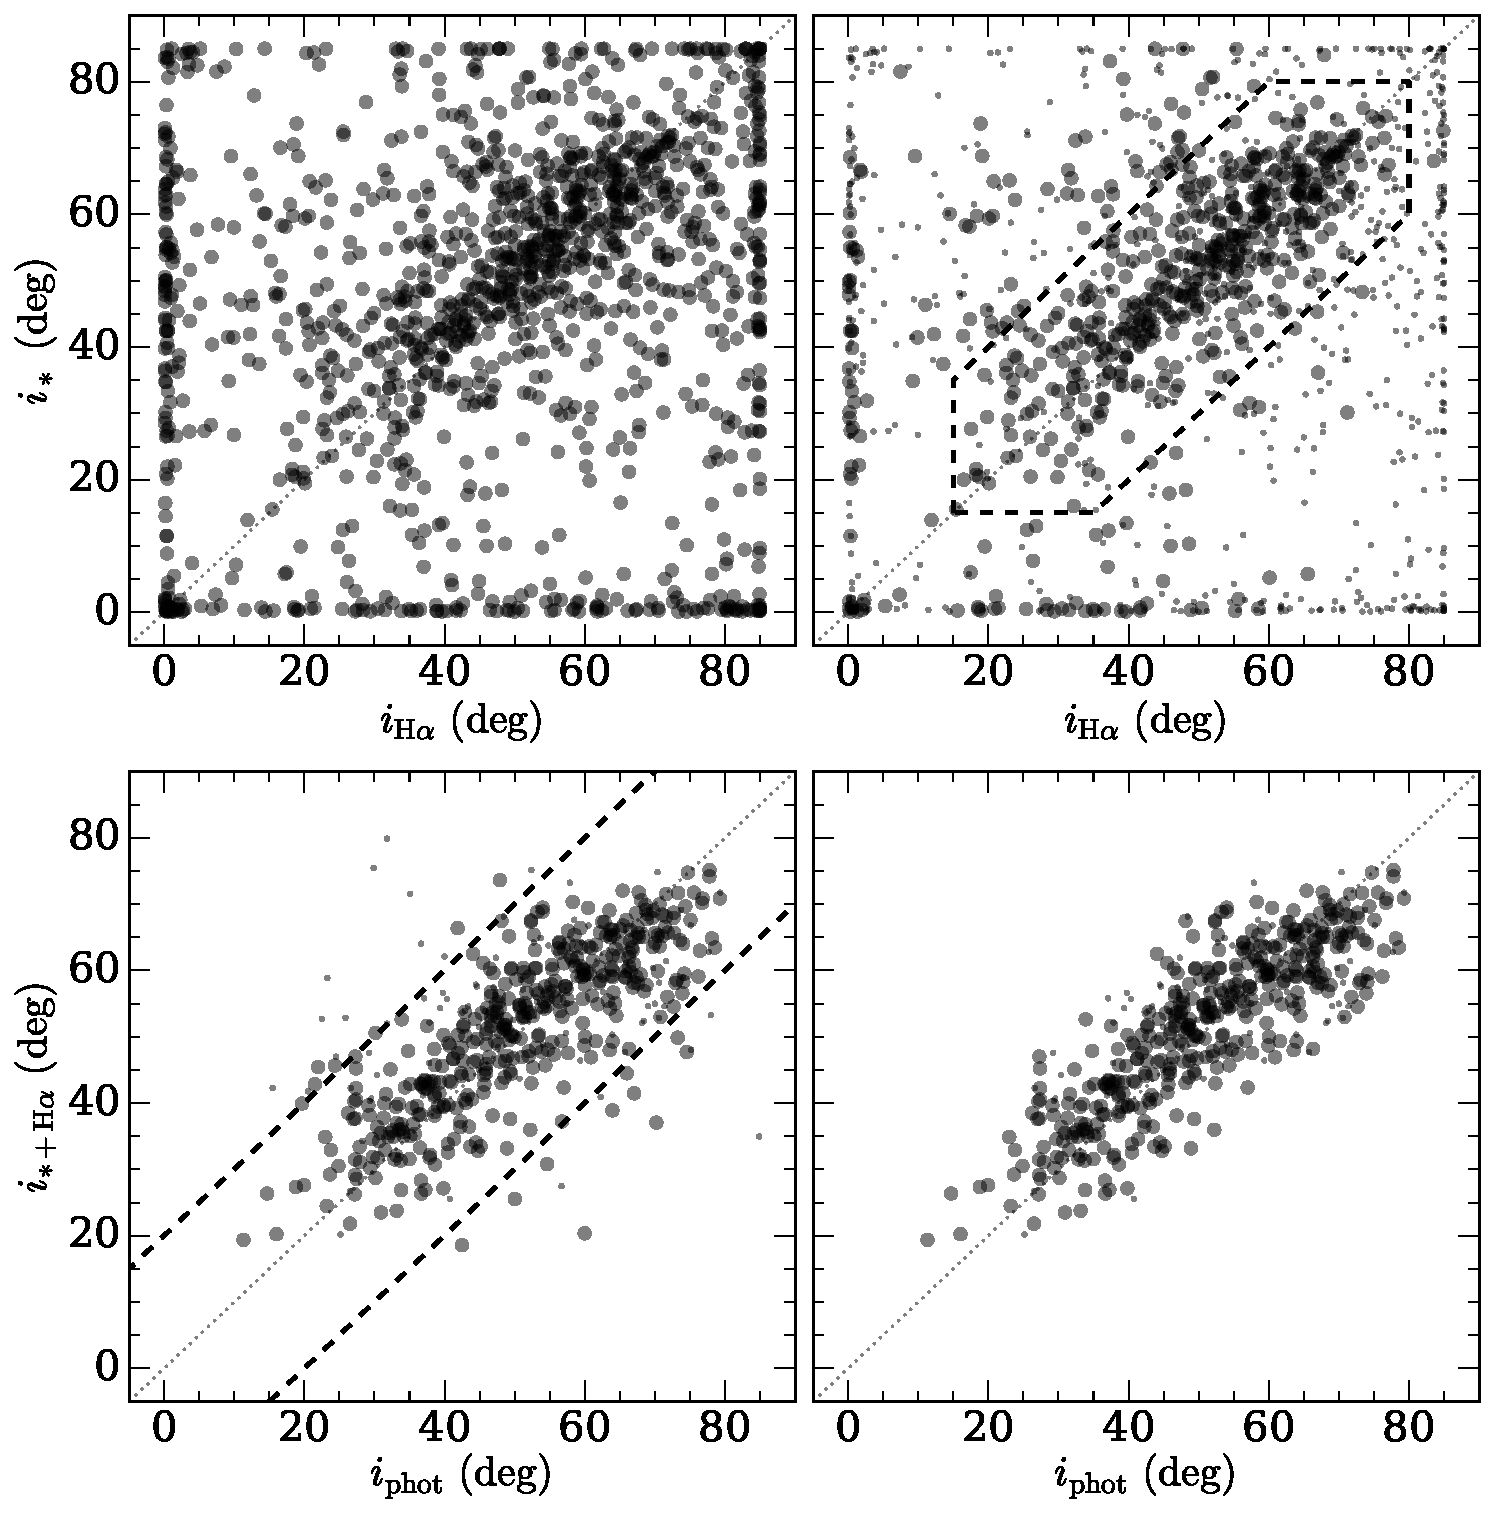
\includegraphics[width=0.98\columnwidth]{figs/inc_select.pdf}
%
\caption{
%
Comparison of the three kinematic inclinations --- as resulting from the
\halpha-only ($i_{{\rm H}\alpha}$), stellar-only ($i_\ast$) and
simultaneous ($i_{\ast+{\rm H}\alpha}$) fits --- with the photometric
inclination, $i_{\rm phot}$ (see eqn.~\ref{eq:inc}).  From top-left to
bottom-right, the panels illustrate the progression of our
inclination-based selection criteria.  The gray dotted line shows the
1:1 correspondence in all panels.  ({\em Top row}): Comparison of
$i_{\ast+{\rm H}\alpha}$ (abscissa) and $i_\ast$ (ordinate) for all 1322
galaxies with successful velocity-field fits.  The top-left panel shows
the distribution before any selection criteria are applied, whereas the
top-right panel converts the point type for galaxies that are {\em not}
selected by the constraints on $V_{\rm sys}$, $(x_0,y_0)$, and $\phi_0$
to small points.  In the top-right panel, the dashed polygon represents
our primary inclination criterion.  ({\em Bottom row}): Comparison of
$i_{\rm phot}$ (abscissa) with $i_{\ast+{\rm H}\alpha}$ (ordinate);
large dots and small points have the same meaning as in the top-right
panel.  The bottom-left panel shows all galaxies that pass our primary
inclination criterion, whereas the bottom-right panel shows only those
galaxies that satisfy both criteria (see text).  The dashed lines in the
bottom-left panel illustrate our secondary inclination criterion.
%
}
%
\label{fig:incselect}
%
\end{figure}

\subsubsection{Inclination}

In Fig.~\ref{fig:incselect}, we compare the photometric inclinations
(see eqn.~\ref{eq:inc}) with the kinematic inclinations determined from
the \halpha-only ($i_{{\rm H}\alpha}$), stellar-only ($i_\ast$), and
simultaneous ($i_{\ast+{\rm H}\alpha}$) velocity-field fits,
illustrating the progression of our inclination selection criteria.

The top-left panel of Fig.~\ref{fig:incselect} shows that the fitted
inclinations for a significant number of galaxies are biased by our
imposed fit boundaries.  Therefore, we first only consider galaxies with
kinematic inclinations that are between $15\degr < i_{\rm kin} <
80\degr$.  Even after imposing this limit, however, we find $i_{{\rm
H}\alpha} - i_\ast \approx -1\degr\pm16\degr$.  The difference between
$i_{\ast+{\rm H}\alpha}$ and either $i_{{\rm H}\alpha}$ or $i_\ast$ has
an understandably smaller scatter of $\pm11\degr$.  If we simultaneously
impose the constraints outlined above for $V_{\rm sys}$, $(x_0,y_0)$,
and $\phi_0$, we are left with 622 of 1322 galaxies that have $i_{{\rm
H}\alpha} - i_\ast \approx -2\degr\pm12\degr$, as shown in the top-right
panel of Fig.~\ref{fig:incselect}.  Based on this distribution, our
primary inclination selection is $15\degr < i_{\rm kin} < 80\degr$ and
$|i_{{\rm H}\alpha} - i_\ast| < 20\degr$.  When applied to fits both
with and without the center fixed, the criterion is satisfied by 524 of
the 1322 galaxies.

Our secondary criterion checks for consistency of $i_{\ast+{\rm
H}\alpha}$ and $i_{\rm phot}$, which is shown in the bottom-left panel
of Fig.~\ref{fig:incselect}.  After imposing only the primary
inclination criterion, we find $i_{\ast+{\rm H}\alpha} - i_{\rm phot} =
0\degr\pm10\degr$; the scatter decreases to $\pm9\degr$ if we also apply
the $V_{\rm sys}$, $(x_0,y_0)$, and $\phi_0$ criteria.  Our secondary
inclination criterion imposes $|i_{\ast+{\rm H}\alpha} - i_{\rm phot}| <
20\degr$, such that the full sample is shown as filled dots in the
bottom-right panel of Fig.~\ref{fig:incselect}.  The combination of the
two inclination criteria yields our most stringent selection cut,
limiting our sample from 1322 to 487 galaxies.

% Since our goal is to measure asymmetric drift, we want to force the
% kinematic geometry fitted to the \halpha and stellar velocity fields to
% be identical; however, we want to allow for the rotation curves of the
% two tracers to be independent.

[[Note the systematic offset between the kinematic and photometric
inclinations at $i_{\rm phot} \gtrsim 60\degr$.  Known inadequacy of the
infinitely thin model.  Check the effect this has on the AD-$\sigma$
distribution.]]

\subsubsection{Summary of selection cuts}
\label{sec:kingeomcuts}

In summary, our AD-$\sigma$ analysis is of galaxies that satisfy the
following set of constraints on the results from the velocity field
fitting:
%
\begin{enumerate}
%
\item When the two velocity fields are fitted simultaneously, the
difference between the systemic velocities fit to the \halpha and stellar
velocity fields must be within -12.5 \kms{} $\leq V_{{\rm
sys,H}\alpha}-V_{{\rm sys},\ast} \leq 17.5$ \kms{} for {\em all} four of
the fit permutations.
%
\item In the two simultaneous fits to the \halpha and stellar data with
the dynamical center left free, the dynamical center must be within half
of the imposed bounding box on the morphological center.
%
\item For {\em all} the relevant fit permutations, the difference
between the \halpha-only and stellar-only fitted position angles must be
less than 15$\degr$.
%
\item In {\em all} six fits when the inclination is freely fit, the
best-fitting kinematic inclination must be in the range $15\degr <
i_{\rm kin} < 80\degr$.  The difference between the \halpha-only and
stellar only kinematic inclinations must be less than $20\degr$ both
with and without a fixed center.  When both tracers are fit
simultaneously, the kinematic inclination must also be within $20\degr$
of the photometric inclination (eqn.~\ref{eq:inc}).
%
\end{enumerate}
%
The simultaneous application of all these cuts yields a sample of 413
galaxies from the original set of 1322.

% (Under the expectation that a similar fraction applies to the full
% MaNGA sample, we should be able to obtain a sample of $\sim$3000
% galaxies for AD measurements in 2020!)

% \subsection{Uncertainties}
% \label{sec:vfuncer}
% 
% \subsubsection{Beam smearing}
% \label{sec:vfbeam}
% 
% [Test by constructing some models?]
% 
% \subsubsection{Template Effects}
% \label{sec:vftpl}
% 
% (Brief) comparison of MILES and MIUSCAT results.
% 
% \subsubsection{Covariance}
% \label{sec:vfcov}


















We model the geometric projection of the rotational plane of each galaxy
using the approach presented by \citep[][see also
\citealt{2011ApJ...742...18W}]{2003ApJ...599L..79A}.  In three
independent fitting iterations, the model fits are optimized for the
\halpha\ velocity field, the stellar velocity field, and simultaneously
for both data sets; for the latter, the geometry is forced to be the
same for the two dynamical tracers, but the parametrized rotation curves
are independent.  We use these velocity-field-fitting results to
objectively isolate a set of ``kinematically regular'' galaxies.
Briefly, galaxies in this sample must have: (i) successful
velocity-field fits for all three approaches, (ii) differences in the
measured \halpha\ and stellar systemic velocity of less than 20 \kms,
(iii) dynamical centers that are consistent to within a fiber diameter
of the morphological center \comment{check the details of this}, (iv)
\halpha\ and stellar velocity-field position angles that are consistent
to within $\pm$15$\arcdeg$, and (v) kinematic inclinations between
$15\arcdeg < i < 80\arcdeg$ that are both consistent between the
\halpha\ and stellar data and with respect to the photometric
ellipticity to within $\pm$20$\arcdeg$.  The constraint on the
inclination is by far the most stringent. \comment{give number of
galaxies cut by each criterion?}  Applying these constraints yields a
sample of 798 observations (for 790 unique galaxies) out of the 2764
observations analyzed.  Eleven galaxies with repeat observations satisfy
the selection criteria; however, only five of these show all
observations are consistently selected.  The remaining six show one or
more of the observations did not pass our constraints \comment{we should
understand why repeat observations are not consistent for the majority
of cases.  low S/N?}.  \comment{Do this or remove the sentence:}
Finally, we also visually inspected the broad-band imaging of these 790
galaxies and eliminated merging and highly extincted (highly inclined)
systems yielding a final sample of XXX galaxies.  We hereafter refer to
galaxies that satisfy our selection criteria as the ``AD sample''.

\comment{limitations of an infinitely thin disk fit?}

Figure \ref{fig:sample} shows the color-magnitude distribution for all
MaNGA galaxies, as well as the distributions of those galaxies included
and excluded from our AD sample.  As expected, galaxies with relatively
high \halpha\ and $r$-band surface brightness are preferentially
selected.  This results in an exclusion of much of the red sequence, as
well as the brightest and faintest galaxies in the blue cloud.  Although
the conclusions we reach based on our AD sample are astrophysically
meaningful, it is important to appreciate that the galaxies in our AD
sample are a biased representation of the overall galaxy population.

\comment{Show histogram of kinematically regular sample against the
volume-corrected distribution of the MaNGA parent sample in Mi and N-r,
and discuss?}

Our velocity-fitting method provides a model rotation curve fit to both
the \halpha\ and stellar data, each parametrized as a hyperbolic tangent
function: $v_{\rm rot} = v_{\rm flat} \tanh(R/h_v)$.  However, our
primary result is based on the error-weighted mean of the deprojected
rotation-curve measurements for each dynamical tracer.  We only include
measurements within $\pm$30$\arcdeg$ of the major axis and construct
radial bins that are $2\farcs5$ wide and centered at 0.25, 0.5, 0.75,
1.0, and 1.25 $R_{\rm eff}$ --- $R_{\rm eff}$ is the effective radius
using the elliptical Petrosian analysis from the NASA-Sloan Atlas.
\comment{Check if the $R_{\rm eff}$ does or does not include the
multiplicative offset to match these Petrosian and Sersic $R_{\rm eff}$
in the mean.}  Specifically, we calculate the error-weighted mean and
standard deviation of $v_j = V_j/\cos\theta_j/\sin i$ and
%
\begin{equation}
%
\sigma_{a,j}^2 = (V_{{\rm H}\alpha,j}^2 - V_{\ast,j}^2) (\cos\theta_j
\sin i)^{-2},
%
\label{eq:dproj}
%
\end{equation}
%
where $V_j$ is the LOS measurement of each component in spaxel $j$
located at the in-plane polar coordinates $R_j$ and $\theta_j$ and $i$
is the disk inclination.

\comment{An example demonstrating the details of our measurements is
illustrated in Figure X.}

We calculate errors in $v_{{\rm H}\alpha}$ and $\sigma_a$ as the
quadrature sum of the error-weighted standard error (i.e., the
error-weighted standard deviation divided by $\sqrt{N}$) and the
propagated error in the error-weighted mean. \comment{Should we revisit
this?  Details of error calculation not all that important.  We're
dominated by intrinsic deviations in the regressions below.}

\section{Results}
\label{sec:results}

%%%%%%%%%%%%%%%%%%%%%%%%%%%%%%%%%%%%%%%%%%%%%%%%%%%%%%%%%%%%%%%%%%%%%%%%
\begin{figure}
%
\begin{center}
%
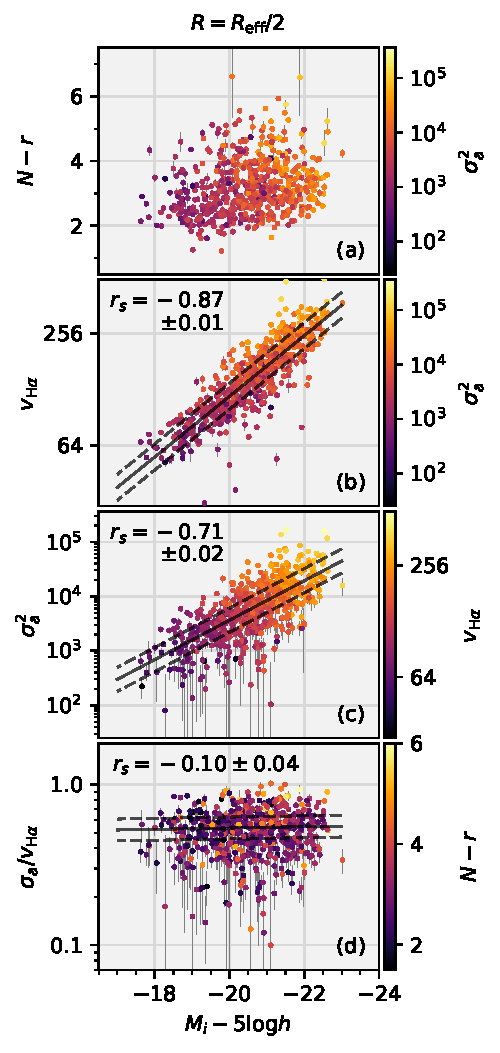
\includegraphics[width=1.0\columnwidth]{figs/mi_models.pdf}
%
\end{center}
%
\caption{
%
Global photometry and kinematic measurements at $R=R_{\rm eff}/2$ for
the AD sample: $M_i$ versus (a) $N-r$ color with each point colored
according to $\sigma_a^2$, (b) $v_{{\rm H}\alpha}$ with each point
colored according to $\sigma_a^2$, (c) $\sigma_a^2$ with each point
colored according to $v_{{\rm H}\alpha}$, and (d) $\sigma_a/v_{{\rm
H}\alpha}$ with each point colored by the $N-r$ color.  Panels (b), (c),
and (d) include the Spearman rank correlation coefficient, $r_s$, and
the linear regressions (solid lines) constructed from the parameters
provided in Table \ref{tab:lines}.  The dashed lines are offset from
linear regression by the modeled intrinsic scatter in the relation
($\varepsilon_y$).
%
}
%
\label{fig:correlation}
%
\end{figure}
%%%%%%%%%%%%%%%%%%%%%%%%%%%%%%%%%%%%%%%%%%%%%%%%%%%%%%%%%%%%%%%%%%%%%%%%

Figure \ref{fig:correlation}(a) shows the $(M_i, N-r)$ color-magnitude
diagram (see right column of Figure \ref{fig:sample}) with the points
colored according to $\sigma_a$ measured at $R=0.5R_{\rm eff}$.  There
is a clear trend where brighter galaxies have larger $\sigma_a$; the
remainder of the Figure examines this trend.

We plot $M_i$ versus $v_{{\rm H}\alpha}$, $\sigma_a^2$, and
$\sigma_a/v_{{\rm H}\alpha}$ in Figures \ref{fig:correlation}(b),
\ref{fig:correlation}(c), and \ref{fig:correlation}(d), respectively.
The points are colored according to the label to the right of each color
bar.  Each panel provides the Spearman rank-correlation coefficient,
$r_s$, of the plotted data with errors derived from $10^3$ bootstrap
simulations.  We have also used a Markov Chain Monte Carlo to sample the
Bayesian posterior distribution for a linear regression to the data in
each panel, incorporating the errors in both axes \citep[see,
e.g.][]{2010arXiv1008.4686H}; the errors in the kinematic quantities
always dominate over the absolute magnitude errors.  The fitted model is
a line in parametric form with an intrinsic Gaussian scatter
perpendicular to the line.  That is, the line is defined as
$\mathbf{l}(t) = \mathbf{l}_0 + t\ \hat{\mathbf{l}}$ for a generalized
coordinate $t$ along the line, an origin $\mathbf{l}_0 = \{x_0, y_0\}$,
and the unit vector $\hat{\mathbf{l}} = \{\cos\phi, \sin\phi\}$.  The
fitted parameters are $y_0$, $\phi$, and the dispersion of the intrinsic
Gaussian scatter about the line, $\varepsilon$; $x_0$ is fixed at the
median abscissa of the data being fitted ($M_{i,0} = -20.6$).  Uniform
priors are used for $y_0$ and $\phi$ and a logarithmic prior
\comment{check this is true} is used for $\varepsilon$
\citep{MacKay:itp}.  Using the returned samples of the posterior, we
also provide parameters for the slope-intercept form of the line --- $y
= mx + b$ where $m = \tan\phi$ and $b = y_0 - x_0 \tan\phi$ --- and the
scatter projected along the ordinate, $\varepsilon_y =
\varepsilon/|\cos\phi$|.  Table \ref{tab:lines} provides the median and
standard deviation of the marginalized distribution of each parameter;
these parameters have been used to construct the lines provided in
Figure \ref{fig:correlation}.

\comment{Show the PDFs?}

%%%%%%%%%%%%%%%%%%%%%%%%%%%%%%%%%%%%%%%%%%%%%%%%%%%%%%%%%%%%%%%%%%%%%%%%
\begin{deluxetable}{ c r r r }
\tabletypesize{\small}
\tablewidth{0pt}
\tablecaption{Linear Regressions for $M_i$ \comment{check m-b form}}
\tablehead{ & \multicolumn{3}{c}{Dependent Variable} \\ \cline{2-4} \\[-3pt]
 \colhead{Parameter} & \colhead{$\log(v_{{\rm H}\alpha})$} &
 \colhead{$\log(\sigma_a^2)$} &
 \colhead{$\log(\sigma_a/v_{{\rm H}\alpha})$} }
\startdata
          $y_0$ &      2.168 &       3.78 &     -0.269 \\
                & $\pm$0.003 &  $\pm$0.01 & $\pm$0.003 \\[2pt]
         $\phi$ &     170.70 &      160.1 &      -0.24 \\
                &  $\pm$0.15 &   $\pm$0.5 &  $\pm$0.17 \\[2pt]
  $\varepsilon$ &      0.069 &      0.209 &      0.068 \\
                & $\pm$0.001 & $\pm$0.005 & $\pm$0.002 \\[2pt] \hline \\[-4pt]
            $m$ &     -0.164 &     -0.362 &     -0.004 \\
                & $\pm$0.003 & $\pm$0.009 & $\pm$0.003 \\[2pt]
            $b$ &      -1.20 &      -3.69 &      -0.36 \\
                &  $\pm$0.05 &  $\pm$0.19 &  $\pm$0.06 \\[2pt]
$\varepsilon_y$ &      0.070 &      0.222 &      0.068 \\
                & $\pm$0.001 & $\pm$0.005 & $\pm$0.002
\enddata
\label{tab:lines}
\end{deluxetable}
%%%%%%%%%%%%%%%%%%%%%%%%%%%%%%%%%%%%%%%%%%%%%%%%%%%%%%%%%%%%%%%%%%%%%%%%

As expected, there is a strong correlation between $v_{{\rm H}\alpha}$
and $M_i$.  However, it is important to note that Figure
\ref{fig:correlation}(b) does not present the
\citet{1977A&A....54..661T} relation for our AD sample; the Figure gives
the rotation speed at $R=0.5R_{\rm eff}$, not a measure of the
full-width of the dynamically broadened line profile.  The slope of the
relation in Figure \ref{fig:correlation}(b) is steeper than a nominal
Tully-Fisher relation because galaxies at low luminosity tend to have
more slowly rising rotation curves \comment{refs}, which can be
confirmed by plotting $h_{v,{\rm H}\alpha}/R_{\rm eff}$ as a function of
$M_i$.  \comment{actually show this?}

Figure \ref{fig:correlation}(c) gives the direct representation of the
gradient in the point color seen in Figure \ref{fig:correlation}(a).
The data in this panel are highly correlated, both as determined by
$r_s$ and the fitted regression.  The intrinsic scatter increases from
0.07 dex (17\%) in $(M_i,v_{{\rm H}\alpha})$ to 0.21 dex (62\%) in
$(M_i,\sigma_a^2)$; however, this is close to the $\sim$0.1 dex scatter
if considering $(M_i,\sigma_a)$ instead.

If $\sigma_a$ or $v_{{\rm H}\alpha}$ was a fully orthogonal secondary
parameter in the distribution of $(M_i,v_{{\rm H}\alpha})$ or
$(M_i,\sigma_a^2)$, respectively, we should expect a gradient in the
point color in Figures \ref{fig:correlation}(b) and
\ref{fig:correlation}(c) {\em perpendicular} to the fitted regression.
However, we see that the primary gradient in point color is parallel to
the fitted regression.  This is consistent with the result that there is
little to no correlation between $M_i$ and $\sigma_a/v_{{\rm H}\alpha}$,
as shown in Figure \ref{fig:correlation}(d):  Both $r_s$ and $\phi$ are
small and only marginally significant with respect to their errors.
From equation \ref{eq:dproj}, this implies that the deprojected stellar
rotation is roughly a constant fraction of the ionized-gas rotation
speed, with $v_{\ast} \sim 0.9 v_{{\rm H}\alpha}$ \comment{give
scatter}.  Although the radius at which the AD was sampled is different,
this ratio is consistent with a similar ratio measured for
DiskMass-Survey galaxies \citep{2013A&A...557A.130M}.

\comment{Need to revisit this paragraph in the context of the
bulge-to-disk fraction.}  The points in Figure \ref{fig:correlation}(d)
are colored by the global $N-r$ color.  It is difficult to determine
from this illustration if their is any correlation between
$\sigma_a/v_{{\rm H}\alpha}$ and global galaxy color.  One might expect
such a correlation if, for example, galaxies with different global color
have different light-weightings of the thin- vs. thick-disk
\comment{refs; not sure there are relevant ones; Comer\'{o}n?}, which
propagates to a difference in which component dominates the dynamical
pressure in the disk midplane.  Figure \ref{fig:colortrend} assesses
this directly by plotting the error-weighted mean trend in
$\sigma_a/v_{{\rm H}\alpha}$ for quartiles of the $N-r$ distribution of
the AD sample.  The error bars represent the error-weighted standard
deviation of the data in each bin, whereas the error-weighted standard
error is always {\it smaller than the plotted point}.  This suggests a
marginal, yet statistically significant, detection of a slightly larger
$\sigma_a/v_{{\rm H}\alpha}$ in the reddest bin.

%; however, more data would be required to lend this result any
%statistical significance.

%%%%%%%%%%%%%%%%%%%%%%%%%%%%%%%%%%%%%%%%%%%%%%%%%%%%%%%%%%%%%%%%%%%%%%%%
\begin{figure}
%
\begin{center}
%
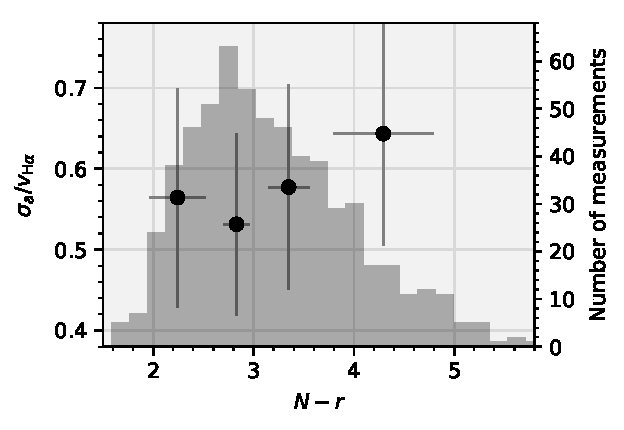
\includegraphics[width=1.0\columnwidth]{figs/adov_vs_color.pdf}
%
\end{center}
%
\caption{
%
The error-weighted mean trend in $\sigma_a/v_{{\rm H}\alpha}$ binned in
quartiles of the global $N-r$ color (black points).  The error bars
represent the error-weighted standard deviation of the data within each
bin; the error-weighted standard error is smaller than the size of each
black point.  The underlying gray histogram provides the number of
measurements in bins of $N-r$; each quartile contains $\sim$152
galaxies.
%
}
%
\label{fig:colortrend}
%
\end{figure}
%%%%%%%%%%%%%%%%%%%%%%%%%%%%%%%%%%%%%%%%%%%%%%%%%%%%%%%%%%%%%%%%%%%%%%%%

\section{Discussion}
\label{sec:discussion}

\subsection{Technical Concerns}

\comment{Sample bias}

\comment{Beam-smearing}

\subsection{Prospects}

\comment{If $\sigma_a$ is a direct proxy for $\sigma_R$ ...}

\bibliography{master}

\end{document}


% Under the nominal assumptions of (i) a radially independent rotation
% speed and SVE shape and (ii) a exponential dispersion profile with an
% e-folding length of twice the disk scale length ($h_R$, ref), equation
% \ref{eq:adformal} can be used to show asymmetric drift will be maximum
% at 1.25$h_R$, or approximately 0.7$R_{\rm eff}$.



%\begin{deluxetable*}{ r r r r r r r r }
%\tabletypesize{\small}
%\tablewidth{0pt}
%\tablecaption{Linear Regressions for $M_i$ [[Check slope-intercept form]]}
%\tablehead{ \colhead{Dependent} & \multicolumn{3}{c}{Parametric Form} && \multicolumn{3}{c}{Slope-intercept Form} \\
%    \cline{2-4} \cline{6-8}
%    \colhead{Variable} & \colhead{$y_0$} & \colhead{$\phi$} & \colhead{$\varepsilon$} 
%                        && \colhead{$m$} & \colhead{$b$} & \colhead{$\varepsilon_y$} }
%\startdata
% $v_{{\rm H}\alpha}$                &      2.168 &    170.70 &      0.069 &&     -0.164 &     -1.20 &      0.070 \\
%                                    & $\pm$0.003 & $\pm$0.15 & $\pm$0.001 && $\pm$0.003 & $\pm$0.05 & $\pm$0.001 \\[2pt]
% $\log(\sigma_a^2)$                 &       3.78 &     160.1 &      0.209 &&     -0.362 &     -3.69 &      0.222 \\
%                                    &  $\pm$0.01 &  $\pm$0.5 & $\pm$0.005 && $\pm$0.009 & $\pm$0.19 & $\pm$0.005 \\[2pt]
% $\log(\sigma_a/v_{{\rm H}\alpha})$ &     -0.269 &     -0.24 &      0.068 &&     -0.004 &     -0.36 &      0.068 \\
%                                    & $\pm$0.003 & $\pm$0.17 & $\pm$0.002 && $\pm$0.003 & $\pm$0.06 & $\pm$0.002
%\enddata
%\label{tab:lines}
%\end{deluxetable*}





Using the photometry from the NSA, Figure \ref{fig:sample} shows the
color-magnitude diagram of all galaxies colored by their mean \halpha\
and $r$-band surface brightness.

However, our nominal approach to measuring the stellar and gas rotation curves will be limited forAs such,
measurements of stellar and/or \halpha\ rotation curves for some systems
will be difficult/impossible.  



\comment{Update this} Although not
excluded from our velocity-field analysis {\em a priori}, we expect to
obtain poor rotation-curve measurements for galaxies with low \halpha\
and stellar surface brightness.

\comment{Extinction corrections for the CMD?}

\comment{Primary vs. Secondary sample?}

